\chapter{Introduction} \label{chap:introduction}

%{\em *** Version: \today~ ***}


Many software applications involve some form of editing: a user views a data structure and provides edit gestures in order to modify this data structure. Different kinds of documents require different ways of editing, and hence a multitude of editors exists, each having its own specific edit model and user-interface conventions. Moreover,  since application designers have different ideas on what constitutes a pleasant edit model, even editors for the same document type may show significantly different edit behavior. Nevertheless, the core edit behavior, whether performed in a word-processor or a spreadsheet, is largely similar: document fragments may be copied and pasted, and new parts of the document may be constructed by selecting from menus or entering text. 

% Although gradually, the edit model and user interface of editors seems to become more standard,
% still many differences exist

An obvious research question is to abstract from the specific aspects of each editor and construct a generic system that can be instantiated to a specific editor application. Building an editor with such a system would require only a fraction of the amount of engineering required to build an editor from scratch. 
% And easy to customize. 
A generic editor enhances consistency between editors, because all instantiated editors share the same edit model, and, furthermore, it facilitates the integration of editors for different document types 


%easy to maintain and develop (features added to generic editor
% work in all applications)..

%(also say a gen editor makes it possible to build editors you wouldn't even
% think of building by hand?)

Especially in the nineteen-eighties, many research projects on structure editing were started. However, the editors developed were generally perceived as being overly restrictive, and attempts at developing less restrictive systems resulted mainly in text-only editors. \nonote{mention syntax-directed/recognizing here already?} Further, regardless of the restrictiveness of the edit model, the applicability of the generic editors was generally limited to source editors for programming languages and simple word-processing applications.
%No generic editor However, no editor gained much popularity . either  applicable or perceived as restrictive.  but not %one has gained widespread acceptance.
In the years following, research interest in structure editing steadily declined, and most of the generic editors that were developed are now used only for educational purposes at the institute of origin.
%Nowadays, the term structure editor even has a rather negative connotation.

In our opinion, the problem with most of these structure editors is that they either focus on editing the document structure, or the presentation (often just text).
%Lambert: (maar welke structuur-editors focussen op de presentatie en niet op de structuur??)
The document-oriented editors may have a powerful presentation mechanism, but poor editing support in the presentation, which results in a restrictive edit model. On the other hand,  purely presentation-oriented editors lack edit operations on the document, and also have relatively weak presentation mechanisms.

With the increasing popularity of the XML format for representing structured documents, the advantages of a powerful generic editor are becoming even more apparent. Many XML document types are being developed, but support for editing documents of these types is still poor. 
% ample support? geeft wel dubbele "there is"
There is a choice between using an expensive custom-made editor, or a generic XML editor, the functionality of which does  not come close to what a presentation-oriented (WYSIWYG) editor could potentially offer. It is not possible to use one of the current XML editors as a convenient editor for a programming language or for mathematical equations.

In response to this situation, we have developed  the presentation-oriented structure editor Proxima. Before we introduce Proxima, we discuss the basic concepts that play a role in editing structured documents. In Section~\ref{sect:introProxima} we introduce the Proxima editor, followed by a summary of the terminology in Section~\ref{sect:terminology} and an overview of the thesis in Section~\ref{sect:overview}.
\bc
In response to this situation, we have developed  the presentation-oriented structure editor Proxima. The editor can be used for a wide range of applications, such as word-processors or source editors, but also equation editing and spreadsheet behavior is possible. The editor has a layered architecture and combines a powerful document presentation mechanism with a non-restrictive edit model. Besides edit operations on the document structure, the editor also allows editing in the presentation.  A platform-independent Haskell prototype has been implemented, and experiments with instantiated editors have yielded promising results.
\ec

\bc para uit advantages of str editors
Despite the advantages mentioned, generic structure editors are not widespread at all. Several structure editors are used in small communities, but most development projects have been terminated, and in the last decade, very few publications on the subject have appeared. The rise of the XML standard has spawned a large number of generic editors, but when regarded as structure editors, XML editors do not show much variation and do not offer many of the possibilities that a structure editor could offer. Hence, their applicability is limited, and using an XML editor to edit a Java program source, for example, is not possible with the current generation of editors.
\ec





%, and provided promising results.

%Not a monolithic system that takes over the entire os. Just an 
%editor for documents.




%								
%								
%								


\bc
Editing is concerned with the creation and maintenance of documents.  
Most documents have some form of structure. 
\ec

\bc uit Xprez
The popularity of the document standard XML has led to an increasing demand for XML editors. The Proxima project is concerned with the design of a generic presentation-oriented XML editor with support for derived values in documents. A presentation is a view on a document, according to a style sheet. In a presentation oriented editor the user only sees a presentation of a document. WYSIWYG editing is possible using a WYSIWYG presentation, whereas the underlying document structure can be viewed and edited with a presentation that shows the actual tags and tree structure of the document. Because Proxima will support derived values, constructs such as chapter numbers and references are not hard-coded in the editor, but can be specified entirely by the user. Also, computations in a document, where one field contains the result of a calculation over several input fields can be modeled with derived values. In order to specify document presentations, a powerful presentation language is required. For this reason, we have developed the declarative XML presentation language {\sc Xprez}.
\ec




%Word documents, HTML, spreadsheet
%
%Vgl sap-centrifuge Oranges bananas peaches
%juicer, blender, ?
%
%1 Juice Tiger. 
%
% only one machine to buy (and develop) to get used to. different extensions different fruits. Easy to mix different juices.
%
%Generic editor, one system one uniform interface. Easy to combine different documents.
%
%Gelaagde architectuur


% Many applications are editing. view document, enter text, copy paste, move parts, navigate. 
% By abstracting over the specifics of the editor, a generic editor could offer a lot of advantages
% Only one editor for a range of documents provides a uniform interface, and makes embedding documents easy.
% moreover XML: lot of specialized documents that require editing. 
% Even though big ones are hard to replace, generic editor can create easily custom editors with advanced functionality

% in the eighties many projects started: Structure editors. Restrictive never popular. Term structure editor is negative.

% Proxima is a generic editor with a number of features that make it possible to apply it to a wide range of applications

% Although the research in this thesis is not specifically tailored for XML, many of the results apply to XML as well, since 
% XML documents are tree-structured documents. 


% identify problems, and propose an architecture with several novel features that .

% ? instead of have formalism for creating fast and safe editors. We want a formalism that allows us to create the editors
% ? we need. Otherwise these have to be built by hand. 

% prototype has been implemented and although still lot of work to do. It already makes it possible to create editors
% in very little time

% maybe borrow from {Why Proxima} section
% also see ch_conclusions


\section{Preliminaries}

\subsection{Structured documents} \label{sect:structdocs}


%\section{Structured documents}
%Basics of XML and DTD's  Schema. CSS. XSL
%XML is EBNF 
%Documents are trees

A {\em structured document} is a collection of logical entities between which a structural relation exists. Examples of structured documents are HTML pages, program sources, word processor documents, etc. 

In this thesis, we restrict ourselves to structured documents that have a tree structure that can be described by an EBNF grammar. Although graphs can be viewed as structured documents as well, algorithms for performing computations over graphs are far more complex than tree algorithms. Furthermore, parsers for graphs are less well understood than parsers for trees, as well as computationally more expensive. 

In cases where we explicitly want to describe the structure of a document fragment, we use monomorphic (i.e.\ parameter free) Haskell~\cite{peytonJones03haskell} data types together with the list type. Example document fragments are represented by Haskell terms. For example, a document representing the let expression  $\mathbf{let}~x = 1;~y = 2~\mathbf{in}~x+y$
\bc $(1+2) \times (3 + 4)$\ec can be denoted in Haskell by: 

\begin{small}
$Let~[Decl~(Ident~\text{``x''})~(Int~1),~Decl~(Ident~\text{``y''})~(Int~2)]~(Sum~(Ident~\text{``x''})~(Ident~\text{``y''}))$
\end{small}
%$Product~(Sum~(Int~1)~(Int~2))~(Sum~(Int 3)~(Int~4))$

\subsection{XML}

The eXtensible Markup Language XML~\cite{xml11} is an increasingly popular standard for representing structured documents. The standard is a simplified descendant of SGML~\cite{sgml86} (Standard Generalized Markup Language). An XML document is a sequence of characters that encodes a tree structure. The nodes of the tree are referred to as {\em elements}. The leaves of the tree are text or attributes (name-value pairs describing properties of an element). The structure of the tree  is represented with opening and closing {\em tags}, and if these tags are nested correctly, the XML document is {\em well-formed}.

The let expression example of the previous section may be represented in XML by:

\ttfamily\begin{small}\begin{tabbing}
<Let><Decl><Ident>x</Ident><Int>1</Int></Decl>\\
~~~~~<Decl><Ident>y</Ident><Int>2</Int></Decl>\\
~~~~~<Sum><Ident>x</Ident><Ident>y</Ident></Sum></Let>
\end{tabbing}\end{small}\rmfamily

%\begin{scriptsize}
%\verb|<Product><Sum><Int>1</Int><Int>2</Sum><Sum><Int val=3><Int val=4></Sum></Product>|
%\end{scriptsize}

The type of an XML document can be specified in several formalisms. The {\em Document Type Definition} (DTD) is part of the XML specification, and basically describes an EBNF grammar over XML elements. A much more expressive formalism is XML Schema~\cite{xmlSchema1}, which itself is a sublanguage of XML. Compared to the DTD formalism, the advantages of using a Schema definition include more control over textual content, as well as a form of inheritance. If an XML document conforms to a certain DTD or Schema, it is called {\em valid}. A third standard, which is not as common as DTDs or Schemas, is the Relax NG standard~\cite{relaxNG01}. Relax NG is a combination of Relax~\cite{relax01} and TREX~\cite{trex01}, and is based on regular expressions. 


%XML is not a meta language.
%Although XML is often referred to as a meta-language, this is not a very accurate term. Indeed, the DTD part of an XML document may %define a language, However, In general, an XML document does not define a language, but is an element of a language. It is only the DTD %description that defines a language. Hence, it would be more appropriate to refer to XML as a super-language.

The number of standards for sublanguages of XML, also referred to as dialects, is rapidly growing. Besides the already mentioned XML Schema, we provide a few more examples.

The Mathematical Markup Language MathML~\cite{mathml20} is a standard for describing mathematical equations and expressions.  \bc Expressions in MathML can be encoded based on  meaning, as well as on presentation. Hence, $1+2$ can be represented either as a sum  element that has two integer child elements, or as a sequence of three elements: two integers with a plus operator in the middle.  \ec Technical documentation can be represented with the DocBook~\cite{walsh02docbook} standard, which exists for XML as well as for SGML. The standard can also be used for papers and books. Finally, we mention the XHTML~\cite{xhtml11} standard, which is an XML encoding of HTML. Although similar, an HTML document is not necessarily an XML document, since HTML is a dialect of SGML rather than XML.


%\note{mention how this thesis relates to XML?}
%** how this thesis applies to XML
%\fromHere

%\verb|<P>Some text with <b>bold</b> and <i>italic</i> words|
%$Para [Text "Some text with", Bold (Text )]$

%Difference between XML and Trees?
%%Difference XML is markup. CFG is tree, everything is part of tree. Markup is more document with tags. leads to differences. 
%things like expressions are awkward to model in XML. On the other hand, mixed... text with bold and bla tags are harder to describe in a %cfg, ...

\subsection{Editing}
\label{sect:editing}


%what is an editor
While the term {\em editor} is usually only associated with plain-text editors such as Emacs~\cite{stallman81emacs} or the ubiquitous Microsoft Notepad, we will use the term in a much broader sense. We regard as an editor any application that presents a visual representation of an internal data structure to a user and allows the user to modify this structure. The internal data structure is referred to as the {\em document} and the visual representation is the {\em presentation}. 

%boundaries of editor concept
Obviously, word processors, image editors, and text editors are editors in this view, but there are also some less obvious examples. Take for example the preferences pane that is part of most window-based applications. The check boxes, selection lists, and text fields can be seen as a presentation of the preferences of the application. Another example of an application that is not usually regarded as an editor is a file browser.


\begin{figure}
\begin{small}
\begin{center}
\begin{center}
~\hspace{1.7cm}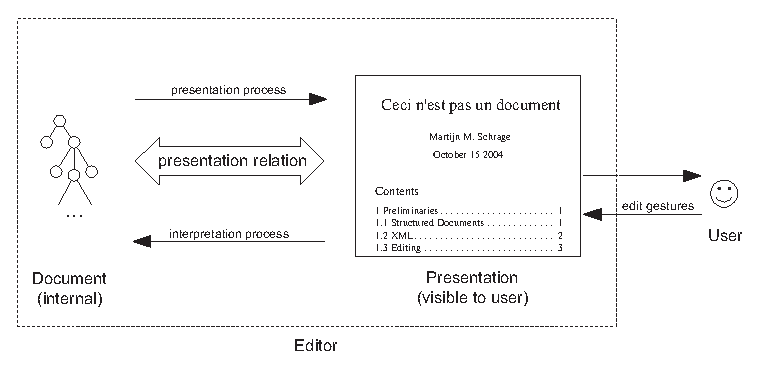
\epsfig{file=pics/eps/editor.eps, width=10cm}
\end{center}\caption{Schematic representation of an editor.}\label{editor} 
\end{center}
\end{small}
\end{figure}

% document and presentation
Figure~\ref{editor} contains a schematic representation of an editor. The main data structures in the editor (also referred to as {\em levels}) are the internal {\em document} on the left that is not visible to the user and the user-visible {\em presentation} on the right. The document should not be confused with a file, which is a representation of the document that is stored on a file system. Furthermore, we also do not consider an XML source to be a document, but rather a textual presentation of the internal document.

\bc define levels \ec

A {\em presentation}, or {\em view}, is the only thing a user sees of the document. A presentation may be textual, graphical, or a combination of both. We focus on static presentations only. Hence, we do not explicitly consider presentations containing sounds or animations, unless presented statically (e.g.\ as a textual link to a sound or video file). In the presentation, the editor shows the focus of attention, or, for brevity, just {\em focus}, which is a shared name for the selection as well the cursor (which is an empty selection).  Several presentations of a single document may be shown simultaneously by the editor, each having its own focus. Finally, if a presentation closely mirrors the final physical appearance of the document when it is printed, it is referred to as a WYSIWYG presentation (What You See Is What You Get).

% what is presenting
The relation between a document and its presentation is denoted by the term {\em presentation relation}, or {\em presentation mapping}. If, according to the presentation relation, the presentation shown to the user is a presentation of the document, we say that the {\em presentation invariant} holds. Computing the presentation of a document is called the {\em presentation process}, whereas computing a document from a presentation is called the {\em interpretation process}. Together, the two processes implement the presentation relation and maintain the presentation invariant if either side of the relation changes.

% what is valid
A presentation is {\em valid} if there exists a document, which, when presented, yields that presentation. A presentation for which there is no corresponding document is invalid. An invalid presentation may result from an editing the presentation level. Note the difference with the term valid document, which denotes a document that is well typed.

\bc
When the presentation level is a presentation of the document, we refer to it as valid. This should not be confused with valid for XML documents which means type correct.
also in defs
\ec

% what is sheet
The presentation relation for an editor may be (partially) specified in a style sheet, or {\em presentation sheet}. A presentation sheet describes how elements of the document type are to be presented, and is a parameter of the presentation process. By modifying the sheet, a user may influence the appearance of the document without having to modify the editor itself. A presentation sheet can be regarded as a parameter to the interpretation process as well, since the interpretation depends on the presentation specified in the sheet. Examples of style-sheet formalisms are the Cascading Style Sheets (CSS)~\cite{css2} for HTML as well as XML, and the Extensible Stylesheet Language (XSL)~\cite{xsl10} for XML.

%what is the editing process
Generally speaking, editing consists of repeated interactive cycles of presenting and interpreting. The editor shows a presentation of the document together with the current focus to the user. The user then provides the editor with an {\em edit gesture}, such as a key press or a mouse movement, which is interpreted as an update on the document. The document is then re-presented and shown to the user. The process is repeated until the user quits the editor. Chapters~\ref{chap:informalSpec} and~\ref{chap:formalSpec} provide a more formal description of the editing process.

\head{Document-oriented versus presentation-oriented editing}

% doc-oriented vs pres-oriented 
Because edit gestures may be targeted either at the document or the presentation, we distinguish two kinds of editing:  {\em document-oriented} versus {\em presentation-oriented} editing.

% also say document editing/presentation editing?

On the one hand, we have {\em document-oriented editing}, which consists of edit operations (including navigation and selection) that are targeted at the structure of the document rather than at its presentation. Examples are swapping two chapters in a word processor, selecting an entire chapter, or navigating to a next section.

On the other hand, {\em presentation-oriented} editing consists of edit operations on the presentation, which do not necessarily make sense at the document level. If a presentation is textual,  presentation-oriented editing amounts to freely editing the text. As an example, take the mathematical expression from Section~\ref{sect:structdocs}: 
$(1+2) \times (3+4)$. Deleting the middle part $(1+\framebox{$\,2) \times ($}\,3+4)$ yields $(1+3+4)$ and is a presentation-oriented edit operation that does not directly correspond to a logical operation on the document level. Another example is navigating downwards in a formatted paragraph of a word processor, since the concept of lines in a paragraph only exists at the presentation level. 

Section~\ref{sect:intrProcess} provides a more thorough discussion of both document-oriented and presentation-oriented editing. Furthermore, the section discusses editing at several other levels, which are introduced at the beginning of Chapter~\ref{chap:proxArch}.
%doc editing is usually also pres editing

\head{Kinds of editors}

%what is structure editor
The term {\em structure editor} is used to make explicit that an editor has document-oriented editing functionality (also including navigation). We do not make a sharp distinction between plain-text editing and structure editing. Instead, we regard all editing as structure editing, but with a varying level of structure. A text editor can be seen as a structure editor with a very simple structure model: a string or a list of strings. Document-oriented and presentation-oriented editing coincide for a text editor.

%what is generic?
An editor is a {\em generic editor} if it is not specifically built for a single document type but can be used to edit a whole class of document types. A generic editor may be {\em instantiated} to yield an editor for a specific document type. Genericity can be achieved with a single generic editor that edits documents of arbitrary types, but also with an editor generator. An {\em editor generator} is an environment that generates an editor application based on descriptions of the document type and its presentation. Although a generator is not as versatile as a single generic editor, we view both as generic editors. 

%structure editor is not nec. generic
For brevity, we will often adopt the common practice that the term structure editor implies genericity as well. Still, structure editors that are not generic are quite common. A few examples are: equation editors, bookmark editors in web browsers, and file browsers. On the other hand, a generic editor is always a structure editor since it knows about the type of the document.


%??maybe introduce XML Editor here? and forward ref?

%who is the user of a generic editor?
In the context of generic editing, the term {\em user} is ambiguous. A user can either be an editor designer, who instantiates the generic editor for a specific domain, or a user who is editing a document. Unless explicitly stated otherwise, we use the term for the document-editing user.


\bc
When regarded as an editor, more sophisticated input fields that incorporate parsers, may be used. Furthermore, normal undo/redo functionality is possible, instead of the course grained OK/Cancel model, which only allows accepting or ignoring all changes at once.
\ec

\bc
% misschien niet zo'n interessante para
With such a broad view of editors, it is possible to regard every application, and even an entire operating system as an editor. In essence, all a computer user does is give edit gestures with the mouse and the keyboard in response to the presentation on the computer monitor. In reaction to the edit gestures, the internal state of the computer changes, giving rise to a new presentation. 

% en nog een
There is no fundamental problem with this view, but we do not adopt it because a definition that is too broad does not help in finding appropriate abstractions for a generic structure editor. Therefore, we do not explicitly consider all applications to be editors, but adopt the view that many applications contain editors.
\ec


Because it is difficult to give a precise definition of a generic structure editor and because such a definition might be restrictive, we will discuss a number of typical use cases to clarify what we mean by a generic structure editor. Section~\ref{sect:usecases} presents these use cases.





%								
\subsection{Advantages of generic structure editors}

An editor that knows about the structure of the edited document can offer interesting\nonote{Doaitse: ``a lot of offer document-type specific'', maar a lot of is niet ok.} functionality. We list several potential advantages of generic structure editors. The first two advantages stem from the genericity of the editor, whereas the rest are mainly about the structural (document-oriented) abilities.

\begin{description}
\item[Uniform user interface/edit model.] Rather than a separate editor application for each type of document, a single generic editor can be used for a range of document types. Thus, instead of having to cope with several slightly different interfaces, a user only needs to deal with a single uniform interface and edit model.

\item[Integration of documents.] Besides offering editors for different types of documents, a structure editor also facilitates the integration of different types of documents into a single editor instantiation. Thus, it is relatively easy to build an editor for a specific document type, with advanced functionality for the different kinds of edit. Examples are a word-processing editor with spreadsheet functionality, or an editor for slide shows that has syntax coloring and type checking for program code appearing in the slides.

\item[Different Views on the Document.] A structure editor may provide a user with several editable views on the document. The views can show the document in a different order, or with a varying amount of detail. 

\item[Graphical Views.] A view may contain color and fonts in order to clarify document structure, but also use layout alignment, and graphical elements such as lines and boxes.

\item[Derived Information in the Presentation.] The editor can analyze the document during editing and display information computed from the document structure. Examples are the results of static analysis and type checking in source editors, but also chapter numbers or an automatically generated table of contents.

\item[Structural Edit Operations.] Some operations, such as demoting a section with subsections to a subsection with subsubsections in a scientific article, are straightforward to specify at the structural level, but awkward at the presentation level.

\item[Structural Navigation.] Navigating over the document structure instead of its presentation can be very useful. In a source editor, when the focus is on an identifier, a user may easily navigate to its definition in the source. Furthermore, an outline view of the document can be shown in which a user can click to navigate to the corresponding position in the document.

\item[Integration with Other Tools.] A structure editor allows fine control over integration with other tools, such as spell checkers, theorem provers, and program-transformation systems. Furthermore, the editor may show the results coming from these tools at the appropriate position in the presentation, rather than as a list of messages with line numbers.


\end{description}

For document types with a textual presentation, such as program sources or XML documents, some of the advantages can be simulated with a text editor. Lexical analysis can be used on the edited text, and basic support for syntax coloring, auto-completion, and navigation can be provided. However, although simple and efficient, these solutions are  very basic and prone to errors, because, in general, much of the structure of a document cannot be recognized at a purely lexical level.

\bc
sometimes basic structural navigation.  Even though some of the document structure can be recognized at lexical level, in the general case, a full parse is needed. For example, when trying to specify a Haskell function definition as a line in which a '=' character is present, also lines containing strings or comments with '=' characters are identified as function definitions. In some cases the problems can be overcome, but in general this amounts to building a parser in a formalism that is too weak for that purpose. Therefore, we will not consider text editors in this overview of editors.
%*********************************
\ec

% maybe say we  explain why this is the case
% maybe say we will change it? or put that in outline?

% pan article




%								
\subsection{Classes of structure editors} \label{sect:classes}

Three classes of structure editors are distinguished in the literature: {\em syntax-directed}, {\em syntax-recognizing}, and {\em hybrid} editors. Syntax-directed editors mainly support edit operations targeted at the document structure, whereas syntax-recognizing editors support edit operations on the presentation of the document. A hybrid editor combines syntax-directed with syntax-recognizing features, but the term is not used consistently. 
%To avoid confusion, we will refrain from using the term hybrid, except in the brief discussion below.

\head{Syntax-directed editors} 
% mention that structure editing is often source editing.

The first structure editors that were developed are the {\em syntax-directed}, or {\em pure}, structure editors~\cite{reps84synGen,Bahlke86PSG,magnusson90orm}.

Early syntax-directed editors show a textual presentation of the document (usually a program source) but exclusively offer edit operations targeted at the internal document structure, and not at the textual presentation. The original idea behind this was that if structural edit operations are available, a user would not need the textual edit operations anymore. Further, presentation-oriented edit operations would interfere with the user's structural model of the document and introduce errors. Hence they were prohibited altogether. Most editors for XML (see also Section~\ref{sect:xmlEditors}), as well as editors for preferences panes, can be regarded as syntax-directed editors.

\begin{figure}
\begin{small}
\begin{center}
\begin{center}
\begin{small}
\noindent \xymatrix@=0.4cm{
   \dataa{$Document$} \ar[dd]    &     \\
                                              & User  \ar[lu] \ar@{.>}[ld] \\
 \dataa{$Presentation$}  &   \\
}
\end{small}
\end{center}\caption{A syntax-directed editor (draft)}\label{synDirEdit} 
\end{center}
\end{small}
\end{figure}


Figure~\ref{synDirEdit} shows a schematic representation of a syntax-directed editor. The editor works by computing a presentation of the internal document structure, which is shown to the user together with a current focus of attention. The user provides an intended edit operation (edit gesture) on the document structure, from which a document update is computed. After the document is updated, a new presentation is computed, which is shown to the user.

If the editor supports clicking in the presentation to set the focus, the editor also needs to keep track of the origin in the document for each position in the presentation.

In the figure, the line between the user and the presentation is dotted because syntax-directed editors do not support edit operations on the presentation very well. Because the presentation is derived from the document, the editor needs to interpret the intended edit operation on the presentation as an edit operation on the document, which is difficult if the edit operation is not a logical operation on the document level.

A major problem with syntax-directed editors is the restrictiveness of the edit model (e.g.~\cite{vanter94practical,rubinNeal87design}). New structures are easy to create, but not as easy to modify. For example, if a user wishes to change a while statement to an if statement, simply typing over the keyword is typically not supported. 

Many later syntax-directed editors offer a form of presentation-oriented editing by providing a freely editable textual presentation of (part of) the document, and applying a parser to the edited text. Some publications~\cite{teitelbaum81progSynth, minor90editing} refer to such editors as hybrid, but, as we will explain below, we still regard these editors as syntax-directed editors. 

Unless the two forms of editing are completely integrated, the textual presentation forces a user to work in a different mode of editing, which is referred to as {\em mode switching}. Mode switching does not solve the problem of restrictiveness adequately. Often, a separate window showing a text-only presentation is opened and before the mode can be switched back, the edited text has to be valid. Furthermore, separate modes require a user to be constantly aware of the current mode of the editor. The resulting increased cognitive burden has been shown to be a source of errors~\cite{sellen90modes}.

% mention problems?
\head{Syntax-recognizing editors} 

At the other end of the spectrum are the {\em syntax-recognizing} structure editors~\cite{budinsky85sre, ballance92pan}. A syntax-recognizing editor keeps track of the textual presentation of the document. The user can freely edit the text, and the editor tries to recognize the document structure by means of a parser. Once the text has been (partially) recognized, structural information (e.g.\ syntax-coloring or type information), navigation, and, in some editors, edit operations are available.

\begin{figure}
\begin{small}
\begin{center}
\begin{center}
\begin{small}
\noindent
\xymatrix@=0.4cm{
   \dataa{$Document$}     &     \\
                                              & User  \ar[ld] \ar@{.>}[lu] \\
 \dataa{$Presentation$} \ar[uu] &   \\
}
\end{small}
\end{center}\caption{A syntax-recognizing editor (draft)}\label{synRecEdit} 
\end{center}
\end{small}
\end{figure}

Figure~\ref{synRecEdit} schematically shows a syntax-recognizing editor. The user's edit operations are targeted at the presentation, which can be edited freely. The document is derived by parsing (interpreting) the presentation; hence the reversed direction of the arrow, compared to Figure~\ref{synDirEdit}.

For each element in the document structure, the editor needs to keep track of what parts of the presentation it corresponds to, in order to show structural information in the presentation, as well as support structural navigation.  When a document structure has been recognized, the presentation may show additional information using font and color changes, context-sensitive menus, tooltips, etc.

Similar to the syntax-directed editor, the picture of the syntax-recognizing editor in Figure~\ref{synRecEdit} also contains a dotted arrow. In this case, because the document is derived from the presentation, structural edit operations on the document are difficult to support. A document-oriented edit operation has to be mapped onto an update on the presentation, in such a way that parsing the updated presentation returns the intended updated document. Presentation information that is not stored in the document tree, such as whitespace and comments, has to be related to the document tree in some way, in order to be put in the right place after a structural edit operation.

The main problem with syntax-recognizing editors lies in their limited applicability. Because the presentation needs to contain enough information to derive the document, interesting presentations that only show part of the document are hard to support. Furthermore, graphical presentations, as well as presentations containing computed values and structures, do not fit the model, as these are difficult to parse. As a result, syntax-recognizing editors are mainly limited to text-oriented applications, such as program-source editors.

% mention: good for program editing?
\head{Hybrid editors} 

The term hybrid editor is used for an editor that supports structural edit operations as well as presentation-oriented (often just textual) edit operations.

In some publications (e.g.~\cite{teitelbaum81progSynth, minor90editing}), the term hybrid is used to refer to syntax-directed structure editors that have a limited form of syntax-recognizing functionality. As a consequence, most syntax-directed editors would qualify as hybrid editors, because most editors support some form of text parsing.

In contrast, other publications (e.g.~\cite{ballance92pan, koorn92gse}) advocate that the term hybrid should be reserved for editors that support full textual editing of the document, as well as limited syntax-directed functionality, even if structural modifications on the document are not supported. In this view, almost all syntax-recognizing editors would classify as hybrid editors, since most of these editors support a form of structural navigation.

%and because of the strictness of the syntax-directed versus syntax-recognizing classification,
Because of the confusion, and because most editors tend to be either primarily syntax-directed or syntax-recognizing, we often use those terms instead.

%Because of this confusion we refrain from using the term hybrid. Instead, we refer to editors that primarily support %document-oriented edit operations as syntax-directed editors, and to editors that primarily support presentation-%oriented editing as syntax-recognizing editors.


\section{Proxima} \label{sect:introProxima}

In this thesis we present the design of the presentation-oriented structure editor Proxima. Proxima can be used for a wide range of applications, including word-processors and source editors, but also mathematical-equation editors and spreadsheets. An important aspect of Proxima is that the editor fully supports presentation-oriented as well as document-oriented editing. Thus, the editor classifies as a hybrid structure editor.

As we mentioned in Section~\ref{sect:classes},  syntax-directed and syntax-recognizing editors generally only have to implement either the presentation or the interpretation mapping. Proxima, on the other hand, supports both  presentation- and document-oriented editing and therefore implements the presentation as well as  the interpretation mapping. 

The implementation of the bi-directional mappings is facilitated by a layered architecture. The computation of the presentation is broken up in several stages, and each intermediate value in this computation corresponds to a {\em data levels} (or just {\em level}). The interpretation process has the same intermediate values. Between two levels, there is a {\em layer}, which takes care of the translations from one level to another, and thus implements a single stage of the presentation and interpretation processes.

\nonote{target intermediate levels}
\nonote{sheets}
%Intermediate levels may also be targeted.

The layered architecture makes it possible\nonote{hoe dan?} to combine presentation-oriented editing with a powerful document-presentation mechanism, which includes the derived values and structures. A platform-independent Haskell prototype of Proxima has been implemented, and experiments with instantiated editors have yielded promising results.


\nonote{toekomst, hier al verschillende levels en layers laten zien, probleem dat presentation dan rendering wordt}
%\begin{figure}
%\begin{small}
%\begin{center}
%\begin{center}
%\begin{small}
%\noindent
%\xymatrix@=0.4cm{
%   \dataa{$Document$}  \ar[dd]   &     \\
%                                            & User  \ar[ld]\ar[lu] \\
% \dataa{$Presentation$} \ar[uu] &   \\
%}
%\xymatrix@=0.4cm{
%   \dataa{$Document (Level_0)$}  \ar[d]   &     \\
%   \dataa{$Level_1$}  \ar[d]\ar[u]   &     \\
%   \dots                                           & User  \ar[ldd]\ar[ld]\ar[lu]\ar[luu] \\
% \dataa{$Level_{n-1}$} \ar[u] \ar[d] &   \\
% \dataa{$Presentation (Level_n)$} \ar[u] &   \\
%}
%\end{small}
%\end{center}\caption{Proxima (draft)}\label{synRecEdit} 
%\end{center}
%\end{small}
%\end{figure}

 
% what about backward mapping, no ES needed? Probably won't know this until some more
% research is done on mappings


\section{Terminology}\label{sect:terminology}

We give a summary of the terms that were introduced in the previous sections.

\begin{description}
\item[Editor:] Application for creating and modifying documents. In this thesis also used to refer to {\em structure editors} and {\em generic editors} (or generic structure editors).
\item[Document:] Internal data structure that represents the information that is edited.
\item[Presentation mapping/relation:] The relation between the document and its presentation.
\item[Presentation-oriented editing:] Edit operation targeted at the presentation: e.g.\ deleting ``\;$+$\;'' from ``$1+2$'', yielding ``$12$''.
\item[Document-oriented editing/structure editing:] Edit operation targeted at the document: e.g.\ swapping two sections in an article.
\item[Presentation sheet:] Parameter to the presentation (and interpretation) process. 
\item[Presentation process:] Process of computing the presentation of a document.
\item[Interpretation process:] Process of computing a document from a presentation.
\item[Level:] Intermediate value of the presentation/interpretation process, also includes document and presentation.
\item[Layer:] Component that realizes the presentation and interpretation between two levels.
\item[Structure editor:] An editor that has knowledge of the structure of the edited document. Usually assumed to be a {\em generic editor} as well.
\item[Generic editor:] A structure editor that is suitable to edit documents of different types.
\item[Syntax-directed editor:] An editor that primarily supports document-oriented editing.
\item[Syntax-recognizing editor:] An editor that primarily supports presentation-oriented editing.
\item[Valid document:] A well-typed document. Mainly used for XML documents.
\item[Valid presentation:] A presentation that is the result of presenting some document.
\item[Focus:] Shared name for cursor and selection.
\end{description} 

%\section{Why Proxima}
%
%(Will be added when all chapters are more or less finished)

%Why proxima
\bc
complex, but:
new stuff:

-extra state
-also editing on all? levels

Document standard XML getting popular, need editors.

interactive transformations, proof editors, rewrite systems
structural data complex presentations: math
programs with types and structural edit ops: IDEs

Proxima not about changing the world: struct editors, views.  editors have illogical/inconsistent features. Easiest to start all over with new model, however will frustrate users. Better to have a model that allow to express the familiar edit models. and merge them seamlessly.
\ec


\section{Outline of the thesis}\label{sect:overview}

The remainder of the thesis has the following structure:

%As mentioned, users regard structure editors as being either overly restrictive, and/or not powerful enough.
Chapter~\ref{chap:requirements} explores applications of generic structure editing by providing five use cases of real-world editors. With these use cases in mind, we formulate a number of functional requirements that in our view are important for a flexible non-restrictive structure editor. We evaluate a number of existing editors according to the requirements, and conclude with an overview of how the Proxima editor is designed to meet the requirements and be able handle all use cases.

The layered architecture of Proxima is introduced in Chapter~\ref{chap:proxArch}.  The chapter discusses the various data levels, as well as the layers that maintain the mappings between the levels. Furthermore,  examples of the presentation and interpretation processes are provided.

In chapters~\ref{chap:informalSpec} and~\ref{chap:formalSpec}, we develop a specification of the Proxima editor. Chapter~\ref{chap:informalSpec} serves as an introduction to the specification and introduces our model of the edit process, as well as the concepts of extra state and duplicates in the presentation. In  Chapter~\ref{chap:formalSpec}, we start by specifying a simple editor, to which extra state and multiple layers are added in subsequent sections. The chapter ends with an informal discussion on how to handle presentations that contain duplicates.

In Chapter~\ref{chap:presenting}, we discuss the {\Xprez} presentation formalism of the Proxima. {\Xprez} is a declarative presentation language, suited for specifying a wide range of presentations. We state a number of requirements for a presentation language for structured documents, and provide an informal overview of {\Xprez} using a series of examples.

A prototype that already offers much of the functionality mentioned in this thesis has been implemented in Haskell. Chapter~\ref{chap:prototype} discussed the implemented prototype and contains screenshots of editors that have been instantiated with it. The chapter also explains which components need to be provided to instantiate an editor.

Finally, Chapter~\ref{chap:conclusions} presents the conclusions and gives an overview of future work.  


\bc
* mention here or in chapter proxArch? (or at all?)
Bootstrapping problem, descr. of levels layers and edit model. second is easier to give with in a formal story. however, design reasons for first are hard to comprehend without idea. So first informal arch and edit model and later the formal stuff


description of architecture combinator chapter:

Chapter~\ref{chap:archCombs} shows how Haskell can be used for describing a layered architecture as developed.
First discuss several methods of realizing connections between layers and abstract from one. Result is combinator library. Chapter ends with application of the combinators for the Proxima implementation.

\ec